\section{Introduction}
\label{sec:introduction}

%% What are soft robots, why are they useful?
\IEEEPARstart{S}{oft} robotic systems have the potential to offer capabilities that go far beyond the repertoire of traditional rigid-bodied robots.
% ; in particular, with regard to safety, robustness, and cost-effectiveness \Ram{the phrase after the semicolon sounds awkward}.
Their compliant structure allows them to adapt their overall shape to navigate unstructured environments, to safely work alongside humans, to manipulate delicate goods, and to absorb impacts without damage \cite{majidi2014soft}. 
Furthermore, soft robotic technology enables designs that are cheap to manufacture and that can be completely encapsulated to provide robust protection from the environment.

\begin{figure}
\centering

\def\picScale{0.08}    % define variable for scaling all pictures evenly
\def\colWidth{0.5\linewidth}

\begin{tikzpicture}
\matrix [row sep=0.25cm, column sep=0cm, style={align=center}] (my matrix) at (0,0) %(2,1)
{
\node[style={anchor=center}] (FREEhand) {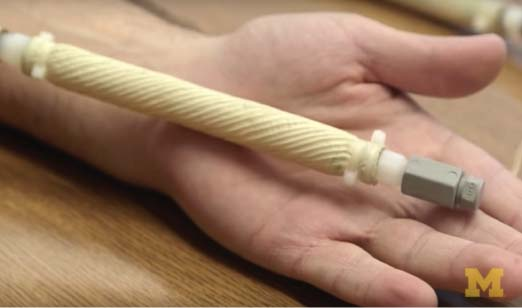
\includegraphics[width=0.85\linewidth]{figures/FREEhand.jpg}}; %\fill[blue] (0,0) circle (2pt);
\\
\node[style={anchor=center}] (rigid_v_soft) {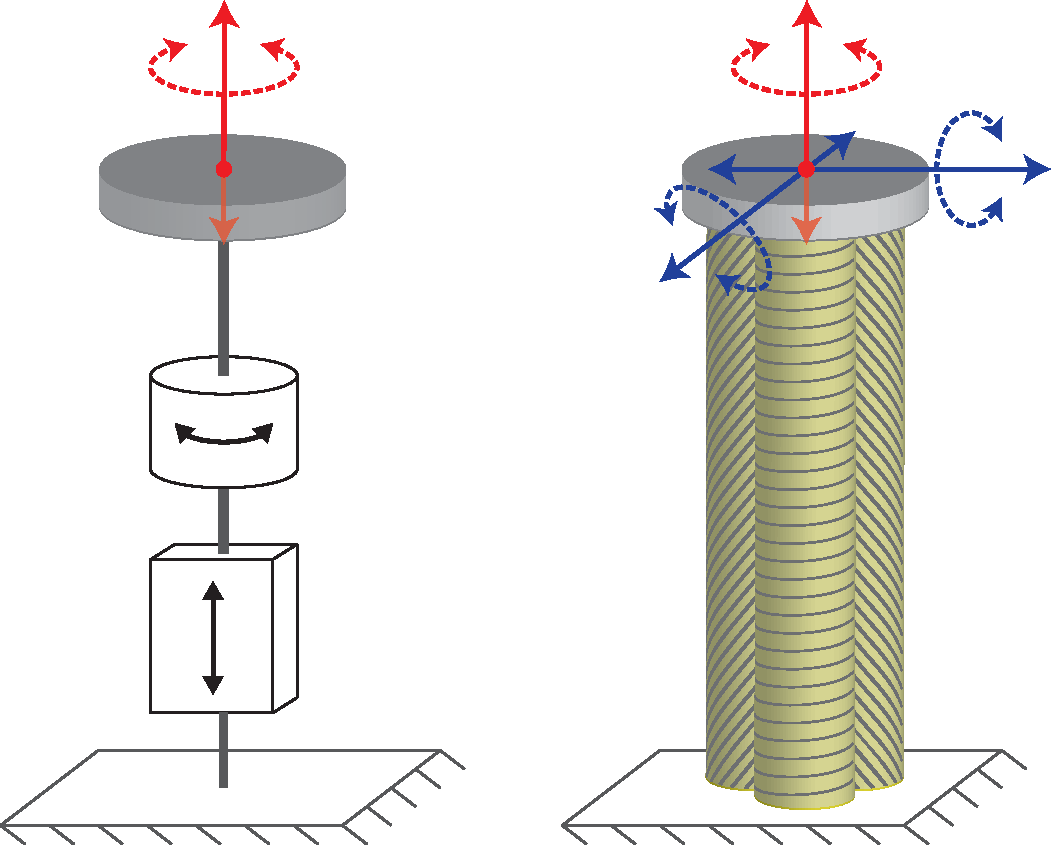
\includegraphics[width=0.75\linewidth]{figures/FREE_vs_rigid-v8.pdf}}; %\fill[blue] (0,0) circle (2pt);
\\
};
\node[above] (FREEhand) at ($ (FREEhand.south west)  !0.05! (FREEhand.south east) + (0, 0.1)$) {(a)};
\node[below] (a) at ($ (rigid_v_soft.south west) !0.20! (rigid_v_soft.south east) $) {(b)};
\node[below] (b) at ($ (rigid_v_soft.south west) !0.75! (rigid_v_soft.south east) $) {(c)};
\end{tikzpicture}


% \begin{tikzpicture} %[every node/.style={draw=black}]
% % \draw[help lines] (0,0) grid (4,2);
% \matrix [row sep=0cm, column sep=0cm, style={align=center}] (my matrix) at (0,0) %(2,1)
% {
% \node[style={anchor=center}] {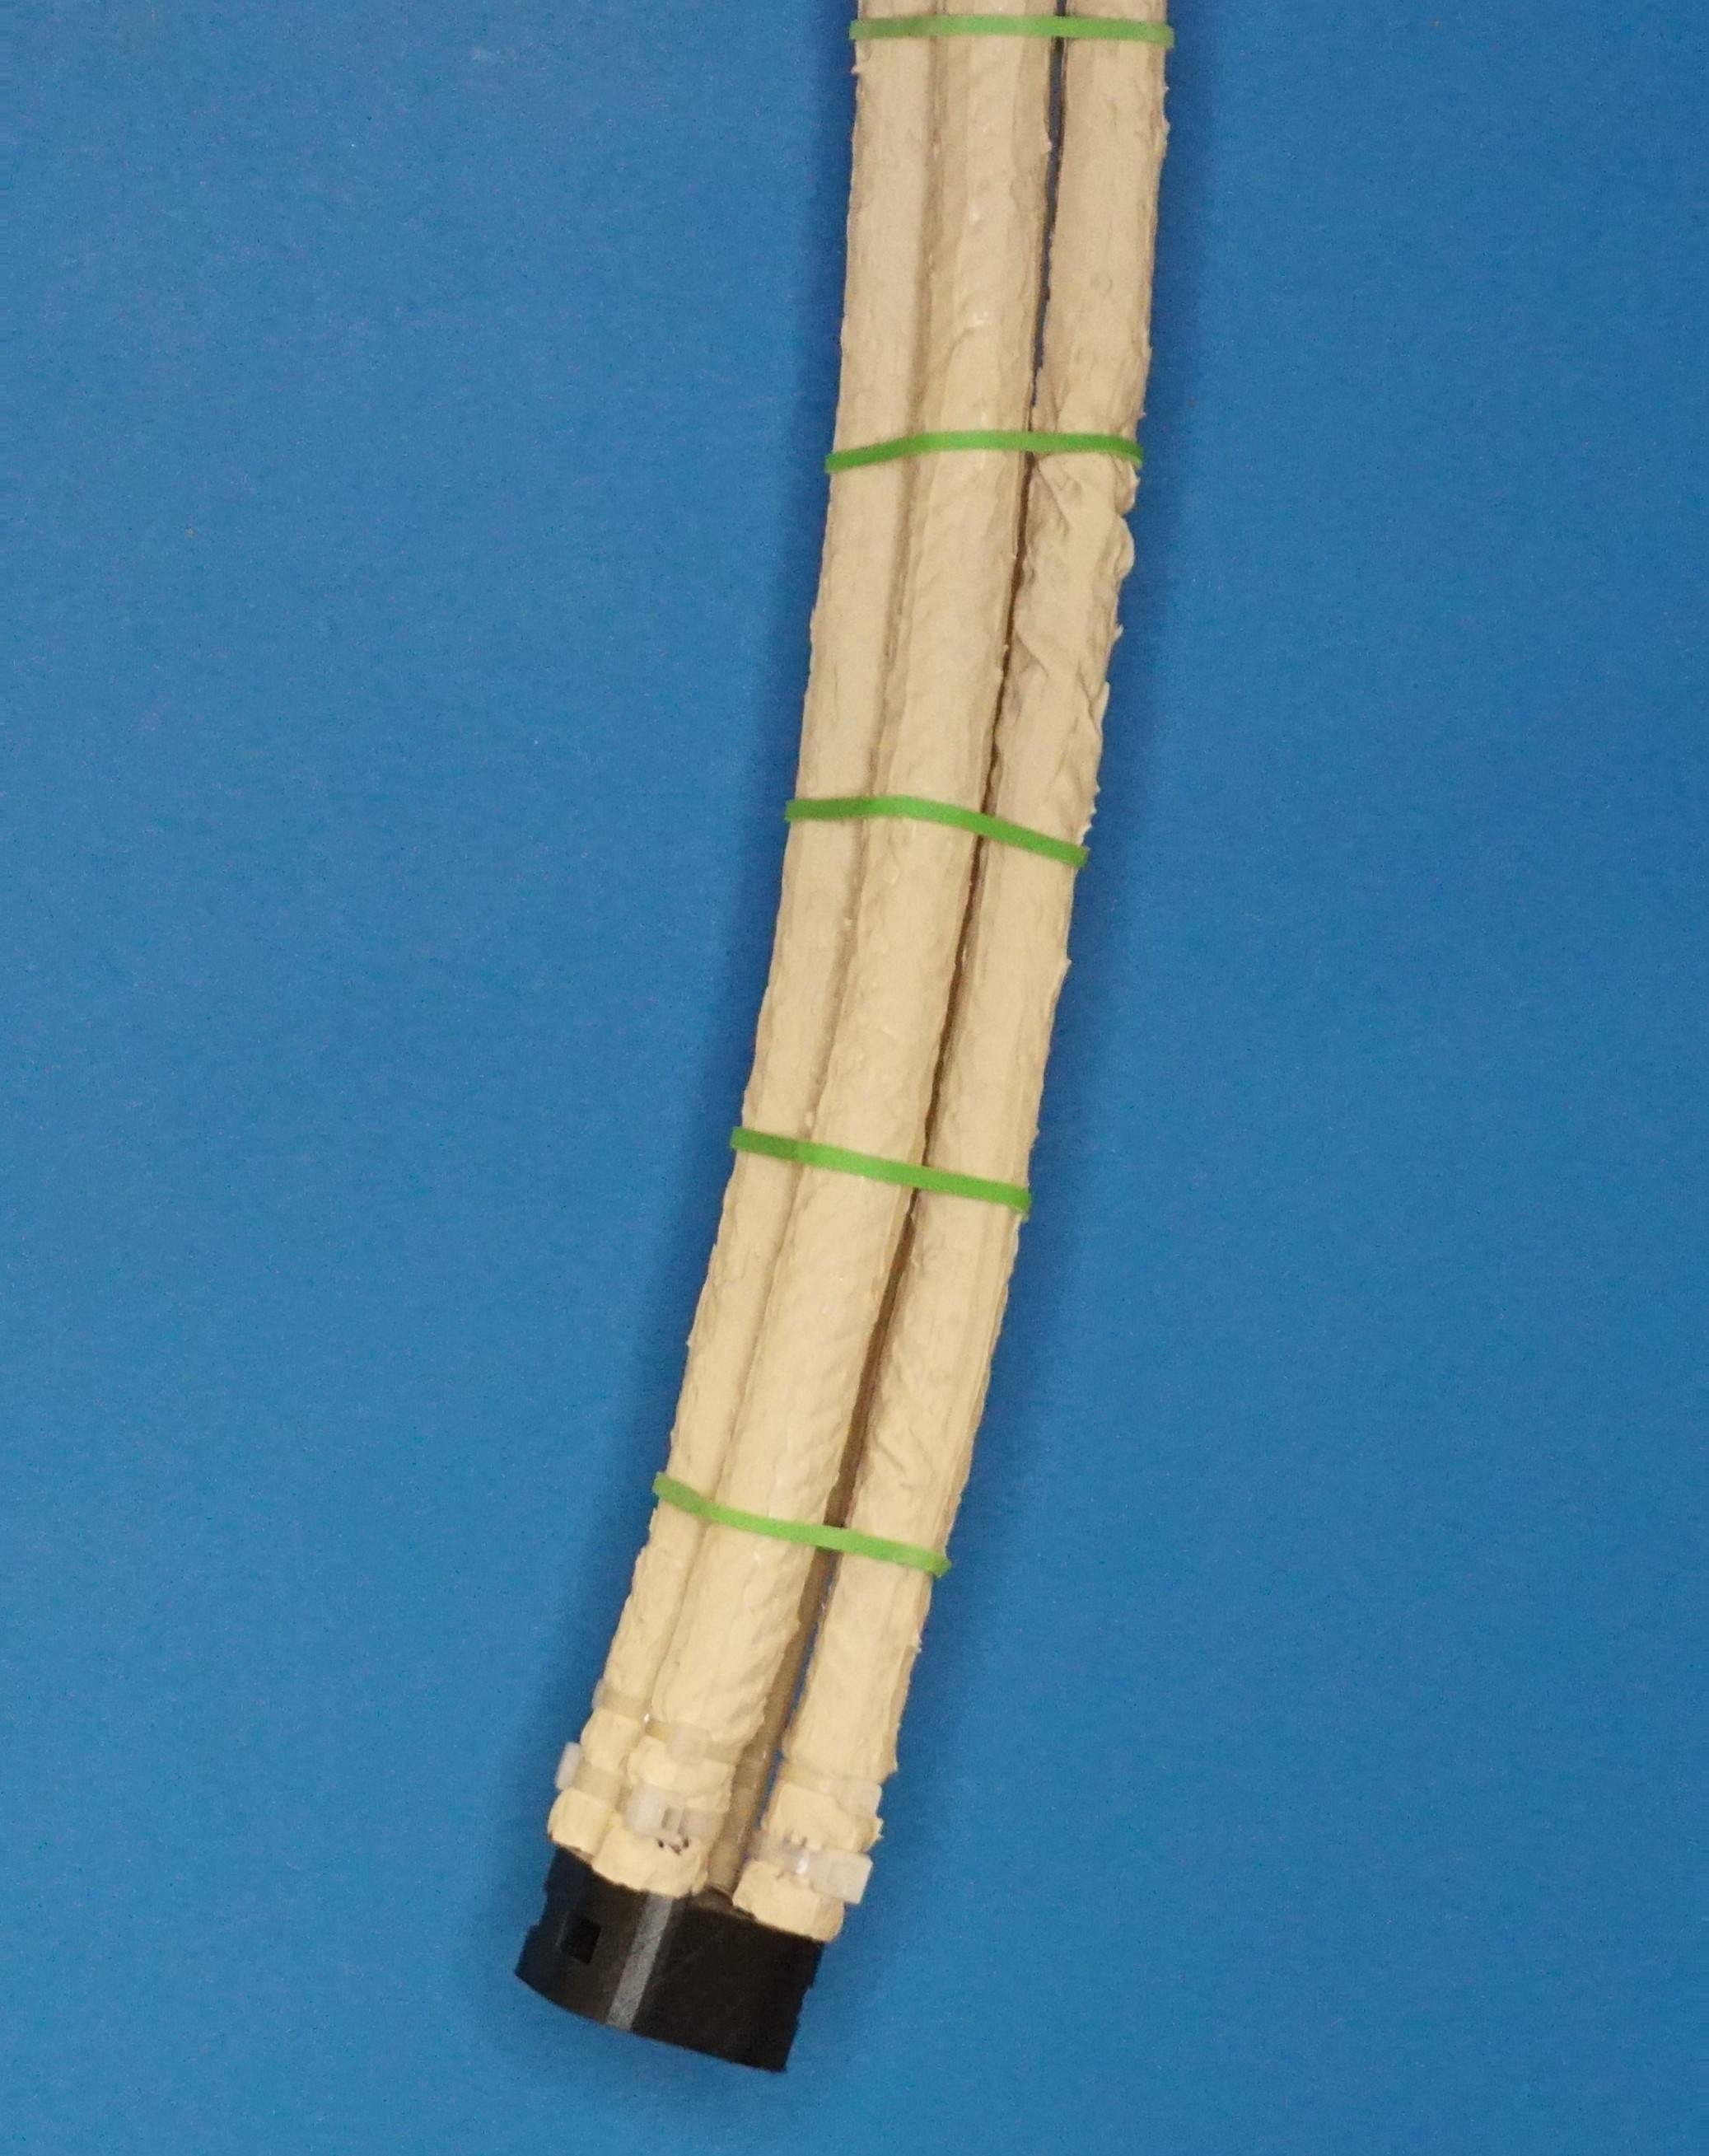
\includegraphics[width=\colWidth]{figures/photos/labFREEs3.jpg}}; %\fill[blue] (0,0) circle (2pt)
% &
% \node[style={anchor=center}] {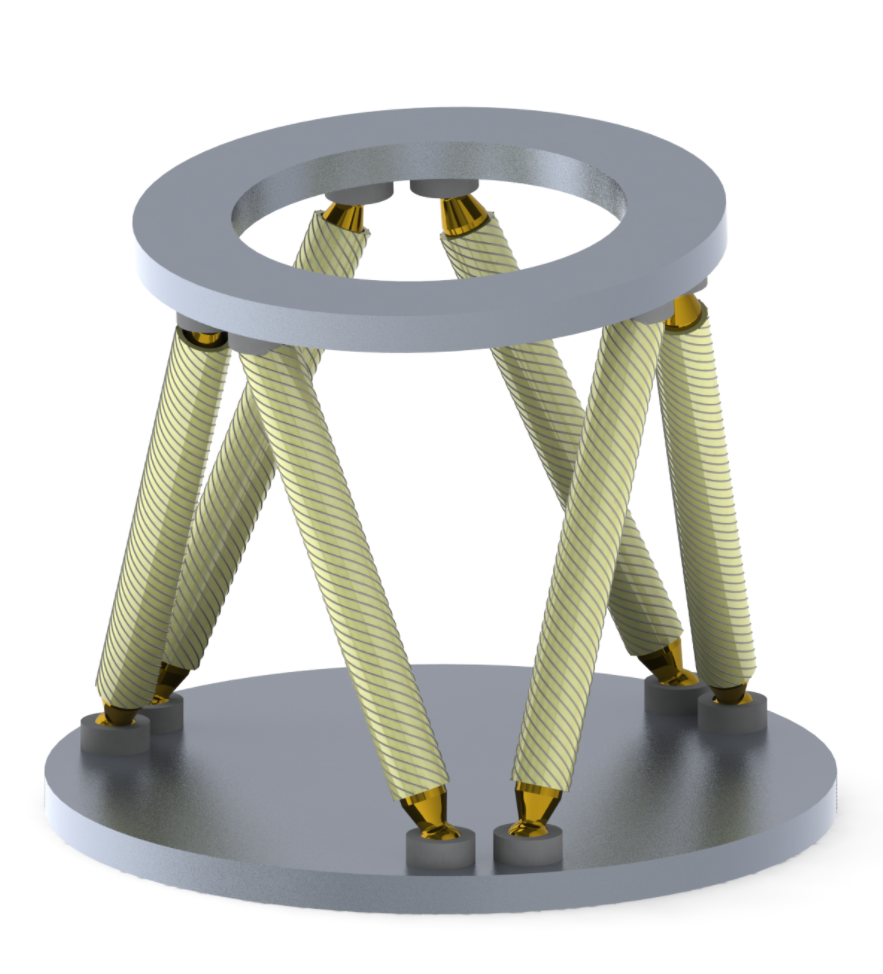
\includegraphics[width=\colWidth, height=160pt]{figures/stewartRender.png}}; %\fill[blue] (0,0) circle (2pt);
% \\
% };

% %\node[style={anchor=center}] at (0,-5) (FREEstate) {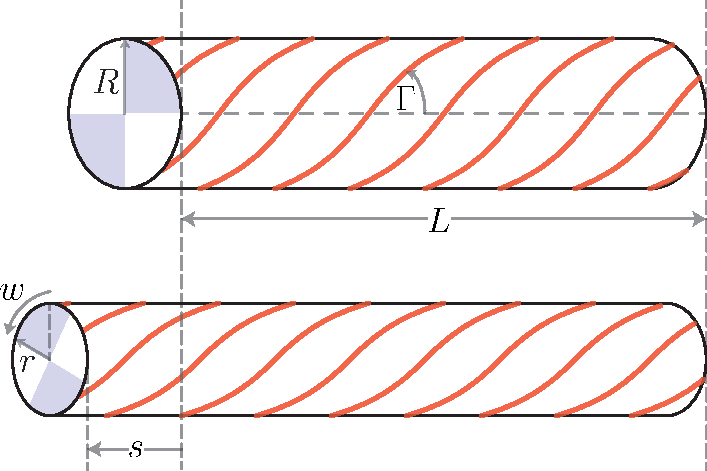
\includegraphics[width=0.7\linewidth]{figures/FREEstate_noLabels2.pdf}};

% \end{tikzpicture}

\caption{\revcomment{2.3}{(a) A fiber-reinforced elastomerc enclosure (FREE) is a soft fluid-driven actuator composed of an elastomer tube with fibers wound around it to impose specific deformations under an increase in volume, such as extension and torsion. (b) A linear actuator and motor combined in \emph{series} has the ability to generate 2 dimensional forces at the end effector (shown in red), but is constrained to motions only in the directions of these forces. (b) Three FREEs combined in \emph{parallel} can generate the same 2 dimensional forces at the end effector (shown in red), without imposing kinematic constraints that prohibit motion in other directions (shown in blue).}}

% \caption{A fiber-reinforced elastomeric enclosure (FREE) (top) is a soft fluid-driven actuator composed of an elastomer tube with fibers wound around it to impose deformation in specific directions upon pressurization, such as extension and torsion. \revcomment{2.3}{In this paper we explore the potential of combining multiple FREEs in parallel to generate fully controllable multi-dimensional spacial forces}, such as in a parallel arrangement around a flexible spine element (bottom-left), or a Stewart Platform arrangement (bottom-right).}

\label{fig:overview}
\end{figure}
   % introductory figure

%% Fluid-driven actuators are a good choice for soft robots
To obtain all of these advantages, it is crucial that every component of a soft robotic system is made in a compliant fashion.
As a result, many soft robotic systems are actuated by fluid-driven soft actuators that can produce forces without imposing a rigid structure \cite{grissom2006design, hawkes2017soft, marchese2014autonomous, tolley2014resilient}. 
In these actuators, a pressurized fluid such as water or air creates a targeted deformation of a soft structure that encloses a fluid-filled cavity. 
To achieve a specific type and direction of deformation, and not merely a homogeneous expansion, the stiffness of the soft structure is pattered in a specific way by adding reinforcing elements such as fibers, beams, or plates \cite{galloway2013mechanically, marchese2015recipe, rus2015design}. 
Examples of these actuators include bellows \cite{pridham1967bellows} McKibben actuators \cite{tondu2012modelling}, and pneu-nets \cite{mosadegh2014pneumatic}.
%, either by the use of inhomogeneous \David{or: `anisotropic'?} materials (cite whitesides, Rus, others from Rus review) or


%% FREEs are great because they are fluid-driven and customizable
A particularly promising type of soft fluid-driven actuator is the fiber-reinforced elasomeric enclosure (FREE) \cite{bishop2015design, krishnan2012evaluating, bishop2013force}, \revcomment{1.7}{also known as the fiber-reinforced soft actuator (FRSA) \cite{galloway2013mechanically, connolly2015mechanical, connolly2017automatic}}.
A FREE consists of a fluid-filled elastomeric tube wound with reinforcing fibers that pattern its stiffness to yield a desired mode and direction of deformation upon pressurization. %(Fig.~\ref{fig:FREEhand}). 
By changing the angles and arrangement of these fibers, a FREE can be customized to yield a large variety of desired deformations and forces \cite{bishop2015design}. 
\revcomment{1.2, 3.5}{This customizability combined with their flexibility and tube-like shape makes these actuators well suited for applications such as a pipe inspection \cite{connolly2015mechanical}, catheter devices \cite{gilbertson2016soft}, or continuum manipulators \cite{grissom2006design}.}



%% Basic argument: Rigid robots: structure constrained, actuators exert forces at joints to move structure,  Soft robots: structure unconstrained, actuators impose forces/constraints to move structure
Due to their soft and deformable structure, FREEs (and fluid driven soft actuators in general) differ in a fundamental way from traditional actuators.
An electric motor, for example, essentially combines a kinematic constraint (the rotation axis of the motor, which is physically defined by a pair of bearings) with a force generating element (the electromagnetic forces, which create the motor torque).
Since the motion of such an actuator is inherently limited to one dimension, multiple actuator stages are typically combined in \emph{series} to achieve multi degree of freedom (DOF) motions (Fig.~\ref{fig:overview}b). 
This is the prevalent design, for example, in industrial robotic arms.
In contrast, in a soft actuator, the force generating element is not supported by any physical kinematic constraints.
The actuator produces a spatial force without constraining the motion to happen exclusively in the direction of this force.
Because of this, soft actuators are particularly well suited to be combined in \emph{parallel}, where the forces of the individual actuators are superimposed to generate a multi-dimensional spatial force (Fig.~\ref{fig:overview}c).
Such parallel combinations enable particularly compact designs of multi-DOF motion stages.
% \Dan{EDIT THIS: They have equivalents in the world of traditional robotic systems, such as the well-known Stewart Platform.
% However, in such systems, the complexity is much higher, as each individual actuator needs to be combined with five additional joints to overcome the inherent kinematic constraints.}


%\begin{figure}
%    \centering
%    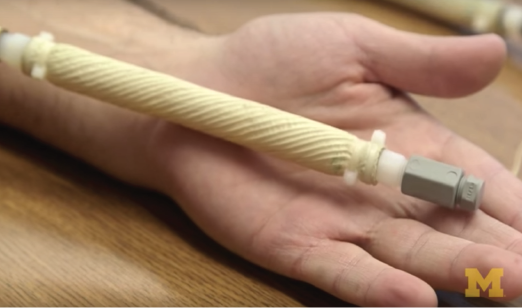
\includegraphics[width=\linewidth]{figures/FREEhand.png}
%    \caption{Possibly just a placeholder, not sure if we can use this image... \David{If you want to make Fig. 1 the overview figure, i would include 4 panels: 1) picture of free (current Fig 1), 2) drawing of free (current fig 3), 3) a parallel combination of frees (i.e., your system) and 4) maybe a steward platform to contrast.}}
%    \label{fig:FREEhand}
%\end{figure}


%% Adaptability of FREEs
One of the benefits of using FREEs as actuators is their mechanical programmability.
% , which makes them particularly well suited for parallel actuator combinations. 
By changing the fiber angle, $\Gamma$, of a single set of evenly distributed parallel fibers (Fig.~\ref{fig:overview}), a FREE can be configured to produce a variety of combinations of forces along its main axis as well as twisting moments about this axis.
The principle behind this adaptability can best be understood by considering a fiber being pulled in a plane (Fig.~\ref{fig:FMratios}a).
For a given fiber force, $T$, the ratio between the $x$ and $y$ components of $T$ is determined by the angle $\Gamma$ (Fig.~\ref{fig:FMratios}b). 
In the case of a FREE, this plane is wrapped into a cylinder (Fig.~\ref{fig:FMratios}c). 
Now the $x$-component of the force pulls along the direction of the central axis of the cylinder, while the $y$-component exerts the twisting moment.
Additional effects, such as the changing radius of the FREE and the fluid pressure acting on its end-caps, make the process a bit more complicated \cite{bruder2017model}, but the ratio between the resulting axial force and twisting moment is fully determined by the fiber angle $\Gamma$ (Fig.~\ref{fig:FMratios}d).

\revcomment{2.2, 2.9}{
A number of researchers have developed ways of modeling fiber-reinforced actuators. Krishnan et. al. characterized the range of achievable motions based on fiber angles \cite{krishnan2012evaluating}, exploring beyond the scope of previous literature which had focused on McKibben actuators only \cite{tondu2012modelling}. Bishop-Moser et. al. formalized a geometry-based kinematic model of FREEs \cite{bishop2015design}, which was subsequently codified and expanded upon by others \cite{felt2018closed, krishnan2015kinematics}. Connolly et. al. took another approach, using finite element methods to predict the motions of fiber-reinforced actuators \cite{connolly2015mechanical}. Bishop-Moser \cite{bishop2013force}, Bruder \cite{bruder2017model}, and Sedal \cite{sedal2017constitutive}, introduced force prediction models based upon the principle of virtual work, force balance, and continuum mechanics, respectively. Furthermore, several papers have been written describing kinematic models of parallel combinations of fiber-reinforced actuators \cite{bishop2012parallel, bishop2012parallelsynth, pritts2004design}.
}

This paper explores the potential of combining different types of FREE actuators in parallel to achieve fully controllable spatial forces, and provides the first generalized kinetic model of parallel combinations of FREEs (to the authors' knowledge).
This work thus expands on the existing literature regarding fiber-reinforced fluid-driven actuators, which has focused mainly on the kinematics or kinetics of individual actuators, or the kinematics of parallel combinations of actuators.
\revcomment{1.5}{While series combinations of FREEs may also be of interest for some applications, that is not the focus of this work.}
Here, we investigate how parallel combinations of FREEs can be configured to enable effective control of multi-DOF forces.
% Here, we study which parallel combinations and configurations of FREEs enable effective control of multi-DOF forces.
To this end, we present a novel way to represent and calculate actuator forces in terms of a state dependent fluid-Jacobian.
% This concept readily extends from a single soft actuator to parallel combinations of actuators.
Our design and modeling methodology is then employed and evaluated experimentally on a two degree of freedom test platform.

% This paper explores the potential of combining different types of FREE actuators in parallel to achieve fully controllable spatial forces.
% This work thus expands on the existing literature regarding fiber-reinforced fluid-driven actuators, which has focused mainly on the kinematics  \cite{bishop2015design, connolly2015mechanical, felt2018closed, krishnan2015kinematics} or kinetics \cite{bishop2013force, bruder2017model, sedal2017constitutive} of individual actuators, \revcomment{1.5}{applications of series combinations of actuators \cite{gilbertson2016soft}}, or the kinematics of parallel combinations of actuators \cite{bishop2012parallel, bishop2012parallelsynth}, \revcomment{2.2}{\cite{pritts2004design}}.
% Here, we study which combinations and configurations of FREEs enable effective control of multi-DOF forces.
% To this end, we present a novel way to represent and calculate actuator forces in terms of a state dependent fluid-Jacobian.
% This concept readily extends from a single soft actuator to parallel combinations of actuators.
% Our design and modeling methodology is employed and evaluated experimentally on a two degree of freedom test bench.

\begin{figure}
\centering

\begin{tikzpicture} %[every node/.style={draw=black}]
% \draw[help lines] (0,0) grid (4,2);
\matrix [row sep=0cm, column sep=0cm, style={align=center}] (my matrix) at (2,1)
{
\node[style={anchor=center}] {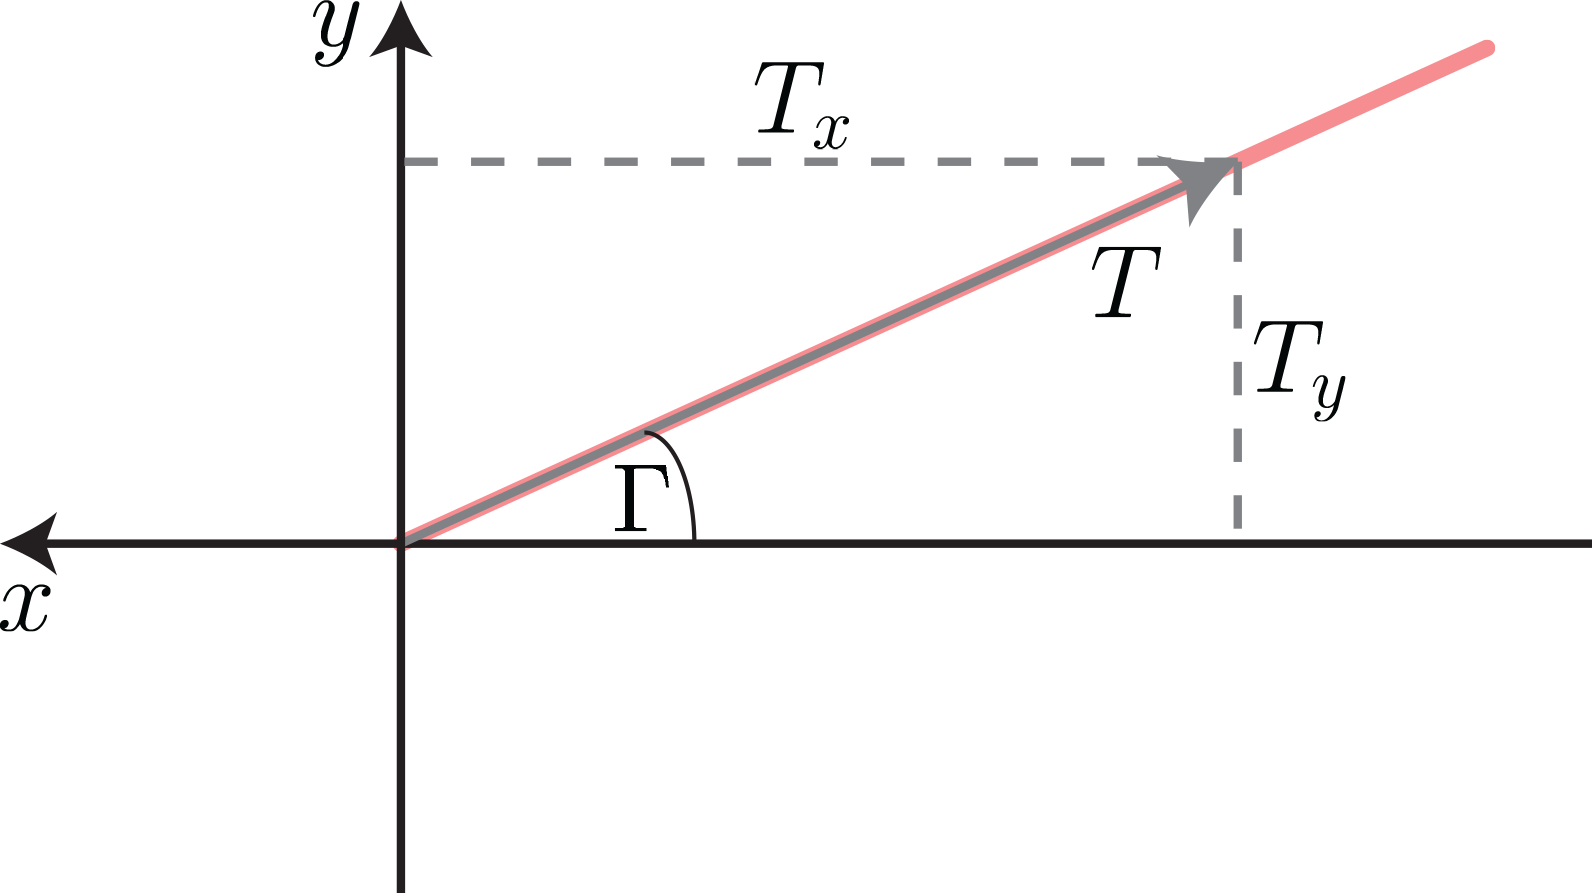
\includegraphics[width=0.42\linewidth]{figures/cableTension.png}}; %\fill[blue] (0,0) circle (2pt);
&
\node[style={anchor=center}] {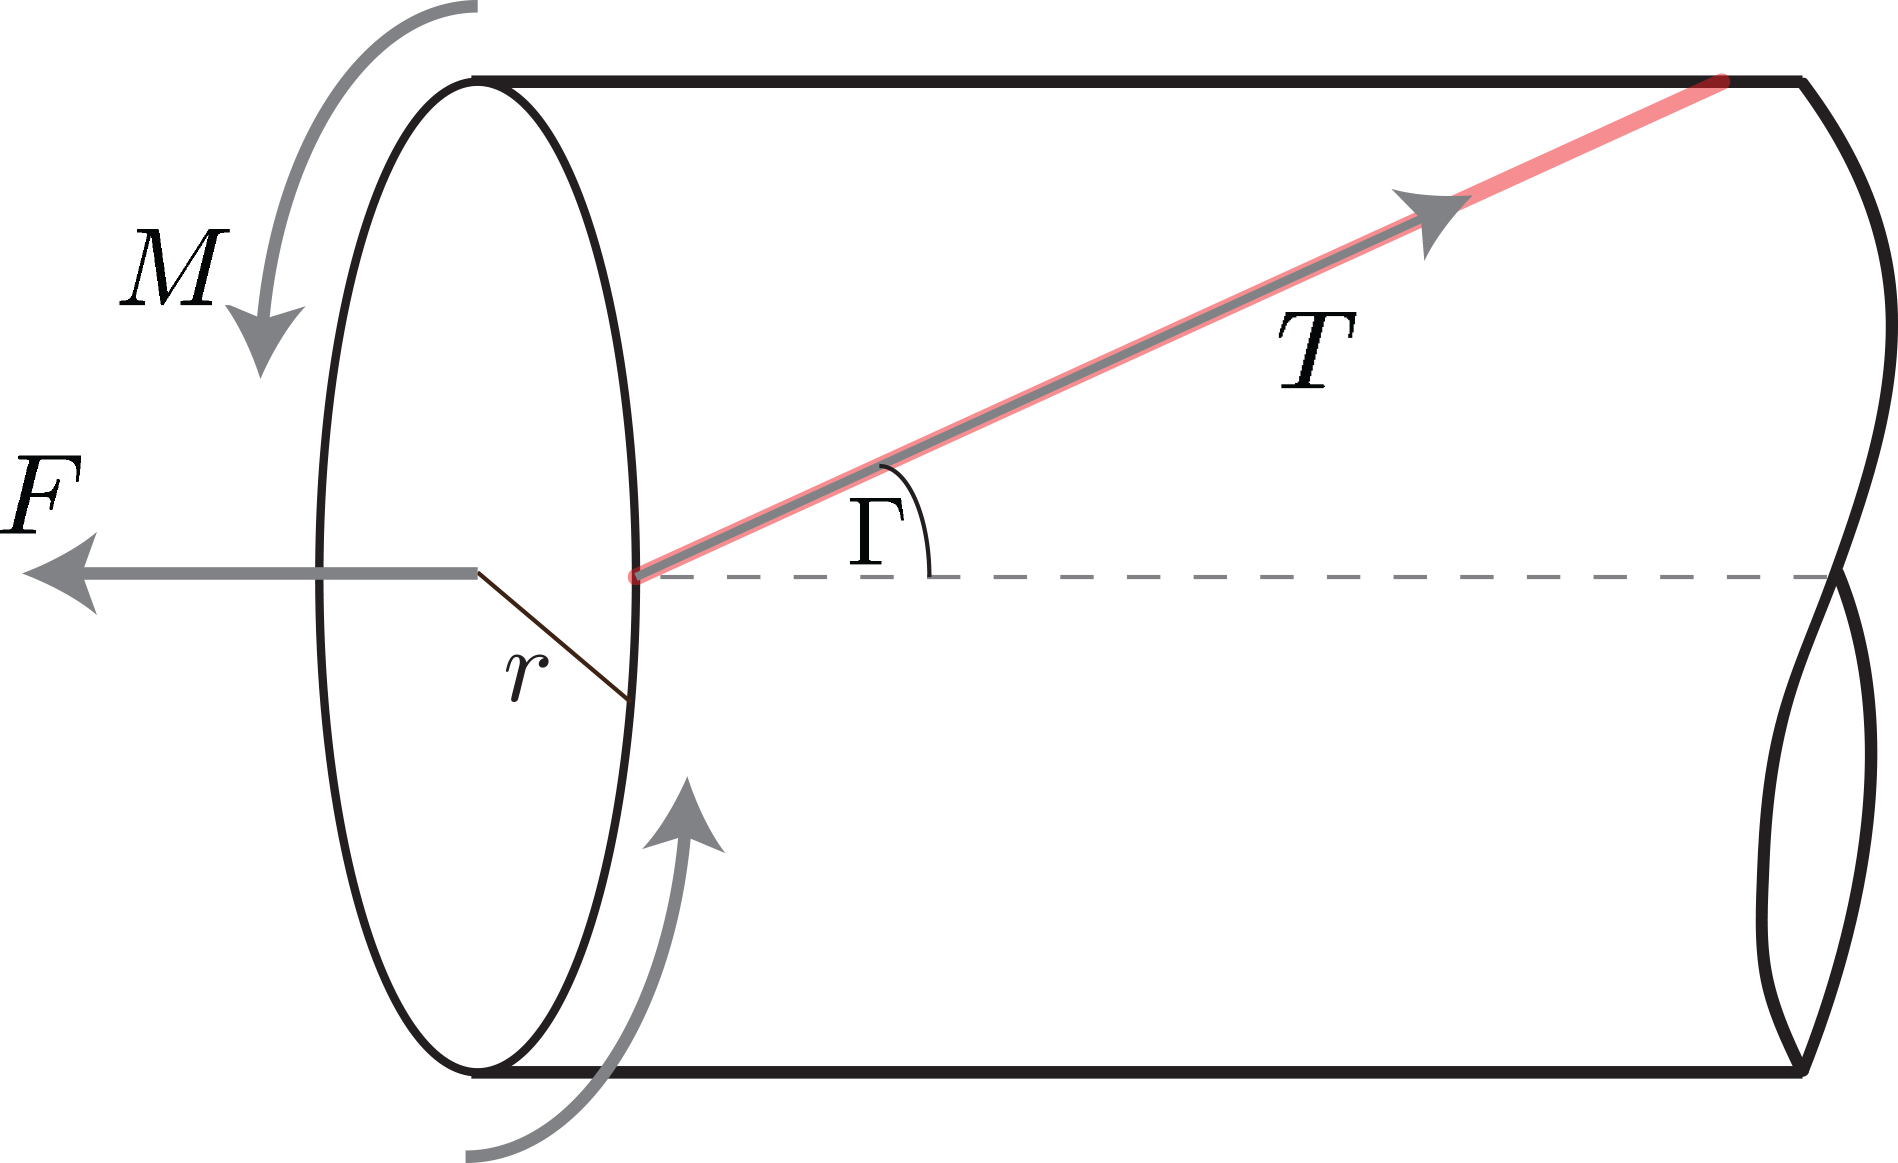
\includegraphics[width=0.42\linewidth]{figures/fiberTension2.png}}; %\fill[blue] (0,0) circle (2pt);

\\
\node (a) {(a)}; & \node (c) {(c)};
\\

\begin{axis}[
    xlabel={\footnotesize{$\Gamma$}},
    ylabel={\footnotesize{$T_x/T_y$}},
    ymin=-10, ymax=10, ytick={0}, ylabel near ticks,
    xmin=0, xmax=90, xtick={0,90}, xticklabel=$\pgfmathprintnumber{\tick}^\circ$, xlabel near ticks,
    tick label style={font=\footnotesize},
    width=0.5\linewidth,
    anchor=center,
]
    \addplot [domain=0:90, dashed] {0};
    \addplot [domain=1:90, samples=100] {-cot(x)};
\end{axis};
& 
\begin{axis}[
    xlabel={\footnotesize{$\Gamma$}},
    ylabel={\footnotesize{$F/M$}},
    ymin=-10, ymax=10, ytick={0}, ylabel near ticks,
    xmin=0, xmax=90, xtick={0,54.7,90}, xticklabel=$\pgfmathprintnumber{\tick}^\circ$, xlabel near ticks,
    tick label style={font=\footnotesize},
    width=0.5\linewidth,
    anchor=center,
]
    \addplot [domain=0:90, dashed] {0};
    \addplot [domain=1:90, samples=100] {(1-2*cot(x)^2) / (2*cot(x))};
    \addplot [mark=none, dashed] coordinates {(54.7,-10) (54.7,10)};
\end{axis};
%\fill[blue] (0,0) circle (2pt);

\\
\node (b) {(b)}; & \node (d) {(d)};
\\
};
\end{tikzpicture}

\caption{By changing the fiber angle of a FREE, it can be configured to produce a large range of force/torque combinations. To understand this, we consider how (a) the angle at which a fiber is pulled in a plane affects (b) the ratio between the $x$ and $y$ components of the pulling force. Similarly, by (c) wrapping the plane into a cylinder and accounting for an internal pressure force pushing out on the endcap, the (d) ratio between axial force and twisting moment can be arbitrarily set by changing the fiber angle.}
\label{fig:FMratios}
\end{figure}











%%%%%%%%%%%% DELETED TEXT BELOW THIS LINE %%%%%%%%%%%%%%%%%%%%%%%%%%%%%%%%%%%%%%%%%%%%%%%%%%%%%%%%%%%%%%%%%%%%%%%%%%%%%%%%%%%%%%%%
\begin{comment}
%% Extrinsic vs. intrinsic actuation
\David{Reading this and the next paragraphs felt a little bit like a detour.  You introduce these two concepts to achieve at the conclusion that a FREE is combining benefits of both.  It reads a bit like you are constructing this case.  Some people might disagree with this classification (there is not citation to support it with literature) and then they won't follow with your conclusions.}
\David{I would propose a more ``positive'' approach in which you don't talk about disadvantages of other systems (this makes you vulnerable for two reasons 1) you piss off people 2) you would need to cover everything else that exists to make your case) but instead just highlight the advantages of yours.}
\David{After starting with one-two paragraph(s) that briefly introduce what soft robots are and why they are useful, I would suggest to focus on fluid-powered systems: ``A large number of soft robotic system are driven by fluid powered actuators \cite{}.  In these actuators, pressurized fluid such as water or air creates a targeted deformation of a soft structure that surrounds a fluid filled cavity.  To achieve a specific type and direction of deformation, and not merely a homogeneous expansion, the stiffness of the soft structure is pattered in a specific way, either by the use inhomogeneous materials \cite{} or by adding reinforcing elements such as fibers, beams, or plates \cite{}.  Examples of these actuators include bellows \cite{,} McKibben muscles \cite{}, ...\cite{}, or ... \cite{}.  The big advantage of these actuators is that they are inherently soft and thus carry all the benefits of soft robotic systems.''}
Current continuum manipulators utilize one of two actuation approaches, intrinsic or extrinsic. Intrinsically actuated manipulators have actuators mounted directly to their backbone, producing forces locally. Soft fluid-driven actuators such as bellows (cite) or McKibben muscles (cite) are popular choices for such schemes due to their ability to produce forces without imposing structure (cite octarm, festo). Extrinsically actuated manipulators, on the other hand, have actuators located off of the manipulator arm itself, and transfer forces to the arm via cables (cite). A benefit of this approach is that it can rely on more conventional actuators such as motors. 

%% Downsides of each type
\David{I would remove this `downside' paragraph it is hard to make it complete.  Instead, focus on the advantages of FREEs}
One downside of intrinsic actuation schemes is that the direction of the forces applied cannot be redirected arbitrarily, since the actuators are mounted directly to the backbone. For this reason, most intrinsically actuated continuum manipulators are adept at producing bending moments, but not twisting. Extrinsic actuation schemes do better in this regard, as cables can be routed and attached to the backbone in ways that produce both bending and twisting moments (cite Clemson, surgical robots). However, cable driven schemes introduce complications such as slack and backlash, which typically require complex mechanical or control systems to remedy \cite{walker2013continuous}.


%% What is a FREE and why it is great.
\David{So rather than saying what the disadvantages of other systems is, focus on why FREEs are good:}
\David{``A particularly promising type of soft fluidic actuators are fiber reinforced elasomeric enclosures (FREEs).  In these actuators an elastomeric fluid-filled tube is wound with reinforcing fibers that pattern the stiffness of the actuator to yield a desired mode and direction of deformation (figure????).  By changing the number, type, and angle of these fibers, FREEs can be customized to yield a large variety of desired deformations.  In particular, for FREEs with a single set of equally wound fibers, changing the angle of the fiber wrapping yields uniquely different combinations of axial forces and twisting torques.''}
The fiber reinforced elasomeric enclosure (FREE) is a type of fluid driven soft actuator that combines the simplicity of intrinsic actuation with the versatility of extrinsic actuation. Composed of an elastomeric tube wound with fibers, FREEs simultaneously exert forces along their central axis as well as moments about that axis \cite{bishop2015design} (see Figure \ref{fig:FMratios}b). This enables FREEs mounted directly to a compliant backbone to produce both bending and twisting moments, without introducing complications like slack or backlash. \David{Not sure if you need the notion of a backbone here...} The ratio between the force and moment produced by a FREE is also customizable, determined by the angle of the wrapped fibers. This unique property of FREEs can be exploited in the design of parallel configurations to generate arbitrary forces at an end effector.

% Explaining the Force/Moment Ratio
In a FREE, fluid pressure is used to induce fiber tension, \David{via the expansion of the elastomeric tube,} \David{remove the parenthesis} therefore the expressions for force and moment in terms of fiber angle are slightly more complicated than in the planar fiber example, as derived and explained in \cite{bruder2017model}
\begin{align}
    \frac{F}{M'} &= \frac{1 - 2 \cot^2{\Gamma}}{2 \cot{\Gamma}}
\end{align}
where $M' = \frac{M}{r}$. Figure \ref{fig:FMratios} illustrates that with a suitable choice of fiber angle $\Gamma$ and radius $r$, a FREE can be constructed with an arbitrary force/moment ratio. It should be noted, however, that as $\Gamma$ approaches $90^\circ$, the magnitudes of force and moment per unit pressure decrease significantly. While it is technically possible to choose $\Gamma$ to produce any desired force/moment ratio, FREEs with lower $\Gamma$ values generate forces much more effectively than those with higher $\Gamma$ values. This implies that FREEs are generally better at producing contractile forces than extensile forces.

For example, a FREE with a single set of evenly distributed parallel fibers exerts a force along its central axis as well as a moment about that axis \cite{bruder2017model}, and changing the angle of the fiber wrapping yields a unique ratio between that force and moment (see Figure \ref{fig:FMratios}b).

\end{comment}


\begin{comment}
% For example, a FREE with a single set of evenly distributed parallel fibers exerts a force along its central axis as well as a moment about that axis \cite{bruder2017model}, and changing the angle of the fiber wrapping yields a unique ratio between that force and moment (see Figure \ref{fig:FMratios}b).
\Dan{Now we can end this paragraph with a nod to the discussion of parallel combinations from above} Furthermore, by arranging FREEs in parallel combinations a wide range of force combinations are possible, making them particularly useful in the actuation of soft structures.

% Basic argument: Rigid robots: structure constrained, actuators exert forces at joints to move structure,  Soft robots: structure unconstrained, actuators impose forces/constraints to move structure
\Dan{I think our discussion of constraints and parallel combinations should be here as a part of the discussion regarding fluidic actuators writ large. Here is my sloppy attempt} A fundamental difference between traditional robots and soft robots is the way actuators interact with structure. Traditional robots are made up of rigid structures connected through joints, and actuators exert forces on these joints to produce desired behavior. Soft robots are made up of non-rigid, compliant structures, and actuators must impose constraints on these structures to produce desired behavior. i.e. the DOFs of a traditional robot are determined by its structure while the DOFs of a soft robot are determined by its actuation. A motor then, is not a suitable actuator for a soft robot, since its rigid structure imposes too many constraints. A fluid-driven actuator, conversely, exerts a constraint only in the direction of actuation, while its soft structure does not inhibit the remaining DOFs of the soft robot. Parallel combinations of fluidic actuators, then, enable the selective constraining of a soft robot to drive its behavior.
\end{comment}